% This is the Reed College LaTeX thesis template. Most of the work
% for the document class was done by Sam Noble (SN), as well as this
% template. Later comments etc. by Ben Salzberg (BTS). Additional
% restructuring and APA support by Jess Youngberg (JY).
% Your comments and suggestions are more than welcome; please email
% them to cus@reed.edu
%
% See http://web.reed.edu/cis/help/latex.html for help. There are a
% great bunch of help pages there, with notes on
% getting started, bibtex, etc. Go there and read it if you're not
% already familiar with LaTeX.
%
% Any line that starts with a percent symbol is a comment.
% They won't show up in the document, and are useful for notes
% to yourself and explaining commands.
% Commenting also removes a line from the document;
% very handy for troubleshooting problems. -BTS

% As far as I know, this follows the requirements laid out in
% the 2002-2003 Senior Handbook. Ask a librarian to check the
% document before binding. -SN

%%
%% Preamble
%%
% \documentclass{<something>} must begin each LaTeX document
\documentclass[12pt,twoside]{reedthesis}
% Packages are extensions to the basic LaTeX functions. Whatever you
% want to typeset, there is probably a package out there for it.
% Chemistry (chemtex), screenplays, you name it.
% Check out CTAN to see: http://www.ctan.org/
%%
\usepackage{graphicx,latexsym}
\usepackage{amsmath}
\usepackage{amssymb,amsthm}
\usepackage{longtable,booktabs,setspace}
\usepackage{chemarr} %% Useful for one reaction arrow, useless if you're not a chem major
\usepackage[hyphens]{url}
% Added by CII
\usepackage{hyperref}
\usepackage{lmodern}
\usepackage{float}
\floatplacement{figure}{H}
% End of CII addition
\usepackage{rotating}

% Next line commented out by CII
%%% \usepackage{natbib}
% Comment out the natbib line above and uncomment the following two lines to use the new
% biblatex-chicago style, for Chicago A. Also make some changes at the end where the
% bibliography is included.
%\usepackage{biblatex-chicago}
%\bibliography{thesis}


% Added by CII (Thanks, Hadley!)
% Use ref for internal links
\renewcommand{\hyperref}[2][???]{\autoref{#1}}
\def\chapterautorefname{Chapter}
\def\sectionautorefname{Section}
\def\subsectionautorefname{Subsection}
% End of CII addition

% Added by CII
\usepackage{caption}
\captionsetup{width=5in}
% End of CII addition

% \usepackage{times} % other fonts are available like times, bookman, charter, palatino

% Syntax highlighting #22
  \usepackage{color}
  \usepackage{fancyvrb}
  \newcommand{\VerbBar}{|}
  \newcommand{\VERB}{\Verb[commandchars=\\\{\}]}
  \DefineVerbatimEnvironment{Highlighting}{Verbatim}{commandchars=\\\{\}}
  % Add ',fontsize=\small' for more characters per line
  \usepackage{framed}
  \definecolor{shadecolor}{RGB}{248,248,248}
  \newenvironment{Shaded}{\begin{snugshade}}{\end{snugshade}}
  \newcommand{\AlertTok}[1]{\textcolor[rgb]{0.94,0.16,0.16}{#1}}
  \newcommand{\AnnotationTok}[1]{\textcolor[rgb]{0.56,0.35,0.01}{\textbf{\textit{#1}}}}
  \newcommand{\AttributeTok}[1]{\textcolor[rgb]{0.77,0.63,0.00}{#1}}
  \newcommand{\BaseNTok}[1]{\textcolor[rgb]{0.00,0.00,0.81}{#1}}
  \newcommand{\BuiltInTok}[1]{#1}
  \newcommand{\CharTok}[1]{\textcolor[rgb]{0.31,0.60,0.02}{#1}}
  \newcommand{\CommentTok}[1]{\textcolor[rgb]{0.56,0.35,0.01}{\textit{#1}}}
  \newcommand{\CommentVarTok}[1]{\textcolor[rgb]{0.56,0.35,0.01}{\textbf{\textit{#1}}}}
  \newcommand{\ConstantTok}[1]{\textcolor[rgb]{0.00,0.00,0.00}{#1}}
  \newcommand{\ControlFlowTok}[1]{\textcolor[rgb]{0.13,0.29,0.53}{\textbf{#1}}}
  \newcommand{\DataTypeTok}[1]{\textcolor[rgb]{0.13,0.29,0.53}{#1}}
  \newcommand{\DecValTok}[1]{\textcolor[rgb]{0.00,0.00,0.81}{#1}}
  \newcommand{\DocumentationTok}[1]{\textcolor[rgb]{0.56,0.35,0.01}{\textbf{\textit{#1}}}}
  \newcommand{\ErrorTok}[1]{\textcolor[rgb]{0.64,0.00,0.00}{\textbf{#1}}}
  \newcommand{\ExtensionTok}[1]{#1}
  \newcommand{\FloatTok}[1]{\textcolor[rgb]{0.00,0.00,0.81}{#1}}
  \newcommand{\FunctionTok}[1]{\textcolor[rgb]{0.00,0.00,0.00}{#1}}
  \newcommand{\ImportTok}[1]{#1}
  \newcommand{\InformationTok}[1]{\textcolor[rgb]{0.56,0.35,0.01}{\textbf{\textit{#1}}}}
  \newcommand{\KeywordTok}[1]{\textcolor[rgb]{0.13,0.29,0.53}{\textbf{#1}}}
  \newcommand{\NormalTok}[1]{#1}
  \newcommand{\OperatorTok}[1]{\textcolor[rgb]{0.81,0.36,0.00}{\textbf{#1}}}
  \newcommand{\OtherTok}[1]{\textcolor[rgb]{0.56,0.35,0.01}{#1}}
  \newcommand{\PreprocessorTok}[1]{\textcolor[rgb]{0.56,0.35,0.01}{\textit{#1}}}
  \newcommand{\RegionMarkerTok}[1]{#1}
  \newcommand{\SpecialCharTok}[1]{\textcolor[rgb]{0.00,0.00,0.00}{#1}}
  \newcommand{\SpecialStringTok}[1]{\textcolor[rgb]{0.31,0.60,0.02}{#1}}
  \newcommand{\StringTok}[1]{\textcolor[rgb]{0.31,0.60,0.02}{#1}}
  \newcommand{\VariableTok}[1]{\textcolor[rgb]{0.00,0.00,0.00}{#1}}
  \newcommand{\VerbatimStringTok}[1]{\textcolor[rgb]{0.31,0.60,0.02}{#1}}
  \newcommand{\WarningTok}[1]{\textcolor[rgb]{0.56,0.35,0.01}{\textbf{\textit{#1}}}}

% To pass between YAML and LaTeX the dollar signs are added by CII
\title{My Final College Paper}
\author{Naomi A. Boss}
% The month and year that you submit your FINAL draft TO THE LIBRARY (May or December)
\date{December 2020}
\division{Mathematics and Natural Sciences}
\advisor{Andrew P. Bray}
\institution{Reed College}
\degree{Bachelor of Arts}
%If you have two advisors for some reason, you can use the following
% Uncommented out by CII
% End of CII addition

%%% Remember to use the correct department!
\department{Mathematics}
% if you're writing a thesis in an interdisciplinary major,
% uncomment the line below and change the text as appropriate.
% check the Senior Handbook if unsure.
%\thedivisionof{The Established Interdisciplinary Committee for}
% if you want the approval page to say "Approved for the Committee",
% uncomment the next line
%\approvedforthe{Committee}

% Added by CII
%%% Copied from knitr
%% maxwidth is the original width if it's less than linewidth
%% otherwise use linewidth (to make sure the graphics do not exceed the margin)
\makeatletter
\def\maxwidth{ %
  \ifdim\Gin@nat@width>\linewidth
    \linewidth
  \else
    \Gin@nat@width
  \fi
}
\makeatother

\renewcommand{\contentsname}{Table of Contents}
% End of CII addition

\setlength{\parskip}{0pt}

% Added by CII

\providecommand{\tightlist}{%
  \setlength{\itemsep}{0pt}\setlength{\parskip}{0pt}}

\Acknowledgements{
I want to thank a few people.
}

\Dedication{
You can have a dedication here if you wish.
}

\Preface{
This is an example of a thesis setup to use the reed thesis document class
(for LaTeX) and the R bookdown package, in general.
}

\Abstract{
The preface pretty much says it all.

\par

Second paragraph of abstract starts here.
}

% End of CII addition
%%
%% End Preamble
%%
%
\begin{document}

% Everything below added by CII
  \maketitle

\frontmatter % this stuff will be roman-numbered
\pagestyle{empty} % this removes page numbers from the frontmatter
  \begin{acknowledgements}
    I want to thank a few people.
  \end{acknowledgements}
  \begin{preface}
    This is an example of a thesis setup to use the reed thesis document class
    (for LaTeX) and the R bookdown package, in general.
  \end{preface}
  \hypersetup{linkcolor=black}
  \setcounter{tocdepth}{2}
  \tableofcontents

  \listoftables

  \listoffigures
  \begin{abstract}
    The preface pretty much says it all.
    
    \par
    
    Second paragraph of abstract starts here.
  \end{abstract}
  \begin{dedication}
    You can have a dedication here if you wish.
  \end{dedication}
\mainmatter % here the regular arabic numbering starts
\pagestyle{fancyplain} % turns page numbering back on

\hypertarget{introduction}{%
\chapter*{Introduction}\label{introduction}}
\addcontentsline{toc}{chapter}{Introduction}

Welcome to the \emph{R Markdown} thesis template. This template is based on (and in many places copied directly from) the Reed College LaTeX template, but hopefully it will provide a nicer interface for those that have never used TeX or LaTeX before. Using \emph{R Markdown} will also allow you to easily keep track of your analyses in \textbf{R} chunks of code, with the resulting plots and output included as well. The hope is this \emph{R Markdown} template gets you in the habit of doing reproducible research, which benefits you long-term as a researcher, but also will greatly help anyone that is trying to reproduce or build onto your results down the road.

Hopefully, you won't have much of a learning period to go through and you will reap the benefits of a nicely formatted thesis. The use of LaTeX in combination with \emph{Markdown} is more consistent than the output of a word processor, much less prone to corruption or crashing, and the resulting file is smaller than a Word file. While you may have never had problems using Word in the past, your thesis is likely going to be about twice as large and complex as anything you've written before, taxing Word's capabilities. After working with \emph{Markdown} and \textbf{R} together for a few weeks, we are confident this will be your reporting style of choice going forward.

\textbf{Why use it?}

\emph{R Markdown} creates a simple and straightforward way to interface with the beauty of LaTeX. Packages have been written in \textbf{R} to work directly with LaTeX to produce nicely formatting tables and paragraphs. In addition to creating a user friendly interface to LaTeX, \emph{R Markdown} also allows you to read in your data, to analyze it and to visualize it using \textbf{R} functions, and also to provide the documentation and commentary on the results of your project. Further, it allows for \textbf{R} results to be passed inline to the commentary of your results. You'll see more on this later.

\textbf{Who should use it?}

Anyone who needs to use data analysis, math, tables, a lot of figures, complex cross-references, or who just cares about the final appearance of their document should use \emph{R Markdown}. Of particular use should be anyone in the sciences, but the user-friendly nature of \emph{Markdown} and its ability to keep track of and easily include figures, automatically generate a table of contents, index, references, table of figures, etc. should make it of great benefit to nearly anyone writing a thesis project.

\textbf{For additional help with bookdown}
Please visit \href{https://bookdown.org/yihui/bookdown/}{the free online bookdown reference guide}.

\hypertarget{lit-review}{%
\chapter{Literature Review}\label{lit-review}}

\hypertarget{survey-methodology}{%
\section{Survey Methodology}\label{survey-methodology}}
\begin{verbatim}
    (2)When you are trying to make asertain something about a population, the most accurate method would be to take data from the entire population. Evaluating the entire population can be cost and time insenstivie. Instead, one may utilize sampling, making an assesment of the population by some smaller part of the population. An important part of conducting a survey is to determine the best method to utilize. Deciding a sample size impacts the precision of the estimate and if the sample is the population, then the estimate is exact. Thus, it is often important to calculate the probability that the estimate is exact.(2)(3) There are two general kinds of sampling: probability and non-probability. The difference between the two is that with probability sampling, a probability of a draw is known. (3)
    - Sampling Procedures
 (1-9)
 
 Probability sampling is used in surveying.
      - Methods (section likely mixed rather than divided like so)
\end{verbatim}
\textbf{Simple Random Sampling}
(1)Simple reandom sampling is a procedure in which you take n independent samples from a population of size N. There are two ways of executing a simple random sample, with replacement and without replacement. If you survey with replacement, every sample has probabiliy 1/N of being drawn. The advantage of surveying without replacement is that you do not have repeated observations in the sample. In finite population sampling a duplicate observation does not provide new information, so it is more usefule to sample without replacement. The samples in the population are still considered indepdent samples; however, since the population decreases by one every draw, the probability becomes \(\frac{n!\text{N-n}!}{N!}\). (1)

(2)When you draw n distinct units of observation(unit) from a population of size N without replacement, it is called \emph{Simple Random Sampling}. Each unit is indepdent of one another with equal probabilty of being drawn. The probability of drawing a specific unit from the population is 1/N. You can use a random number generator on a computer to determine which units to include in your sample. Since each unit has equal probability of being drawn, the population mean is the average of the observations:
\[
\mu = \frac{1}{N} \left(x_1 + x_2 + \cdots + x_n \right) = \frac{1}{N} \sum^{N}_{i=1} x_i
\]
with a population variance of
\[
\sigma^2 = \frac{1}{N-1} \sum_{i=1}^{n} \left(x_i - \mu \right)
\]

Similarly, sample mean and variance are:
\[
\overline{x} = \frac{1}{n} \left(x_1 + x_2 + \cdots + x_n \right) = \sum_{i=1}^{n}x_i 
\]
\[
s^2 = \frac{1}{n-1} \sum^n_{i=1} \left( x_1 - \overline{x} \right)^2
\]

You can also calculate the variance of the estimators themselves. If you use the population variance, you derive the variance of the estimator:
\[
\text{var}\left(\overline{x}\right) = \left(\frac{N-n}{N}\right)\frac{\sigma^2}{n} 
\]
If you use the sample variance, then you get an unbiased estimator of the variance:
\[
\widehat{\text{var}}\left(\overline{x}\right) = \left(\frac{N-n}{N}\right)\frac{s^2}{n}
\]
A variation of simple random sampling takes samples withoutreplacement. The draws are still independent of one another, but repeated observations is now allowed. This is used in situations where you do not want repeated observations. Now, instead of each draw being equal proability, we have that every sequence of samples is of equal probability. This slightly alters the sample mean
\[
\overline{x}_n = \frac{1}{n}\sum^n_{i=1}x_i
\]
with a variance of
\[
\text{var}\left(\overline{x}_n\right) = \frac{1}{n\space N} \sum_{i=1}^N\left(x_i = \mu\right)^2 = \frac{N-1}{n\space N}\sigma^2
\]
The unbiased estimator of the variance of the sample mean is
\[
\widehat{\text{var}} \left( \overline{x}_n \right) = \frac{s^2}{n}
\]
(2)
\textbf{Stratified:}
(1)Stratified random sampling is a variation of sampling in which you partition the population into disjoint subpopulations that you sample from. The overall outcome of the survey is the combination of independent probability samples taken from the disjoint groups. There are several reasons why stratified random sampling can be advantageous. Stratified sampling can provide more precise estimates, especially if your aim involves comparing subgroups. Moreover, it allows flexibility in the method of conducting the surveye by customizing for each strata.(1)

(2)Another method of sampling is called stratified sampling, where you separate the population into disjoint subpopulations algorithmically. Then you can sample from each strata independenty. You can combine the mean and variations of each strata to caluclate the total variance and mean of the sample. One goal when designing the partition, is to minimize the variance within each strata. If the sampling procedure of each strata is simple random sampling, then the method is referred to as stratified random sampling. Both the sample mean and the \emph{i}th observation are random variables
Here we can define elements and probabilities for stratified sampling. Let \emph{h} refer to a specific strata, with the population partitioned into \emph{L} stratas. Let us define the terms and variables associated with stratified sampling.
Let h be a designator of the strata. The total population size is the sum of the sizes of each strata, \(N_h\). The sample size is the sum of the samples taken from each strata, denoted \(n_h\). We define \(\tau\) as the sum of the unit values in the population, and \(\tau_h\) to be the sum of the unit values in strata \emph{h}. The population mean is \(\mu/N\) and the mean of each strata is \(\mu_h = \tau_h/N_h\).
Let \(\hat{\tau}_h\) be the unbiased estimator of \(\tau_h\). The unbiased estimator of the population is
\[ \hat{\tau}_{st} = \sum^L_{h=1}\hat{\tau}_h \]
The variance of this estimator is the sum of the variances of the strata estimators:
\[
\text{var}\left(\hat{\tau}_{st}\right) = \sum^L_{h=1}\text{var}\left(\hat{\tau}_h\right)
\]
with an unbiased variance is similarly equal to the sum of the unbiased variances of each strata.
Regardless of sampling method, we can define the stratified estimator of the mean to be
\[
\hat{\mu}_{st} = \hat{\tau}_{st}/N
\]
The unbiased variance of the estimator, given that the sample selection from each strata are indepdent, is
\[
\widehat{\text{var}} \left( \hat{\mu}_{st} \right) = \frac{1}{N^2} \sum^L_{h=1} \hat{\text{var}} \left(\hat{\tau}_{st}\right)
\]
(2)
\textbf{Cluster:}
\emph{M}: total number of seconary units
\emph{N}: the number of primary units
\emph{M\_i} total number of secondary units in the \emph{i}th primary unit
\(x_i\): the total of the values in the \emph{i}th primary unit
\(x_{ij}\): the \emph{j}th secondary unit in the \emph{i}th primary unit
\(\tau\): population total of secondary units
\(\mu\): population mean per secondary unit
\(\mu_1\): population mean per primary unit
\(\hat{\tau}\): unbiased estimator of population total
\(\text{var}(\hat{\tau})\): variance of the unbiased population total estimator
\(\sigma^2_u\): variance of the primary unit totals
\(\widehat{\text{var}}(\hat{\tau})\): unbiased estimate of the variance
\(s_u^2\): sample variance of the primary unit totals
\(\hat{\tau}_r\): ratio estimator of population total
\emph{r}: sample ratio
\(p_i\): probability of draw proportional to \emph{i}th primary unit size.

(1)Cluster sampling is similar to stratified sampling because both methods involve segmenting the primary population; however, the choice for how the population is split is different. A unit is included in the sample if it falls within the partition of the cluster. When calculating probabilities, you need to consider how many clusters there are, as well as how many units are within each cluster. A cluster sample can be advantageous because it is cheaper to conduct than other methods. Moreover, populations are often distributed in natural clusters such as comparing universities. (1)

(2)The structure of cluster sampling and systemic sampling is the same. First the population is partitioned into units called \emph{primary units}. Within each unit was have \emph{secondary units}, or the units of observations. The primary unit of a cluster sample is determined by spacing proximity. On the other hand, the primary unit of a systemic sample is determined by equally spaced secondary units. The key aspect of cluster sampling and systematic sampling is that you choose the sample by selecting primary units, therefore, all secondary units in a primary unit will be included in the sample. There is variability in characterisitics of the primary units in cluster sampling, such as size and shape, which can provide supplementary information but can affect the efficiency of the sample.

The selection of primary units is conducted by other sampling procedures.You can use simple random sampling to select a primary unit. Calculating the unbiased estimators using simple random sampling without replacement:
Estimator of population total
\[
\hat{\tau} = \frac{N}{n}\sum^n_{i=1} = N\overline{y}
\]
where \(\overline{y} = (1/n)\sum^n_{i=1}y_i\) is the sample mean of the primary unit totals. Let \(\sigma^2_u\) be the finite population variance of the primary unit totals
\[
\sigma^2_u = \frac{1}{N-1}\sum^N_{i=1}(y_i-\mu_i)^2
\]
Then the variance of the population total estimator is
\[
\text{var}\left(\hat{\tau}\right) = N\left(N-n\right)\frac{\sigma^2_u}{n}
\]

and an unbiased variance is
\[
\widehat{\text{var}}\left(\tau^2\right) = N\left(N-n\right)\frac{s^2_u}{n}
\]
\(s^2_u\) is the sample variance of the primary unit totals, calculated by
\[
s_u^2 = \frac{1}{n-1}\sum^n_{i=1}\left(y_i-\overline{y}\right)^2
\]

The ratio estimator based on size can be more efficient than simple random sampling. The primary unit totals for cluster sampling do not have to be the same size, so the unit total is highly correlated to unit size. The sample ratio \emph{r} is defined as
\[
r = \frac{\sum_{i=1}^n x_i}{\sum_{i=1}^n M_i}
\]
Then the ratio estimator of population total is
\[
\widehat{\tau}_r = rM
\]
You can approximate the variance or mean squared error of the ratio estimator
\[
\text{var} \left( \hat{\tau}_r \right) \approx \frac{N(N-n)}{n(N-1)} \sum_{i=1}^N
\left( x_i - M_i\mu \right)^2 
\]
which has an estimator
\[
\widehat{\text{var}} \left( \hat{\tau}_r \right) \approx \frac{N(N-n)}{n(N-1)} \sum_{i=1}^n
\left( x_i - rM_i\right)^2 
\]
The population mean per primary unit is calculated by dividing the ratio estimator by the number of primary units. (2)
\begin{enumerate}
\def\labelenumi{(\arabic{enumi})}
\item
  Systemactic sampling is a specific kind of cluster sampling. First decide on the number of samples n. Choose a random number between 1 and the number of clusters, this will (1)
\item
  The Hansen-Hurwits estimator is a cluster sampling method which proportionalizes the probability of drawing the primary unit based on the size. The unbiased Hansen-Hurwitz estimator is
  \[
  \hat{\tau}_p = \frac{M}{n}\sum^n_{i=1}\frac{x_i}{M_i}
  \]
\begin{verbatim}
  - Advantages/Disadvantages
  pg 255
  Unequal sampling - chp 6
  pg 49
  113-125
\end{verbatim}
  \begin{itemize}
  \tightlist
  \item
    Data Collection
    \begin{itemize}
    \tightlist
    \item
      Designing survey (sample unit, sample size, hypothesis/motivation role)
      pg 247
      pg 258
      31-33
    \item
      Survey method (brief list e.g.~interview, questionnaire)
    \end{itemize}
  \item
    Data Analysis
    \begin{itemize}
    \tightlist
    \item
      Hypothesis testing
    \item
      Inference
    \end{itemize}
  \end{itemize}
\end{enumerate}
\hypertarget{non-probability-sampling}{%
\section{Non-Probability Sampling}\label{non-probability-sampling}}
\begin{verbatim}
 - Sampling Procedures
      - Methods
           - Convenience sampling
           - Consecutive sampling
           - Judgmental Sampling
           -Hansen-Hurwitz 
           46-49
      ##Advantages/Disadvantages
 - Data Collection
      - Designing Survey (sample unit, sample size, hypothesis/motivation role)
      - Survey method (brief list e.g. interview, questionnaire)
 - Data Analysis
 67
 94-99
      - Hypothesis testing
      - Inference
      
\end{verbatim}
\hypertarget{election-polling}{%
\section{Election Polling}\label{election-polling}}
\begin{verbatim}
 - Purpose
 - Design
      - Population
           - Sample selection
      - Methods
      - Sample size
      - Question design
           - Wording impacting response
 - Data collection
      - Implementation
      - Errors
           - Sampling Error
           - Non-Sampling Error
                - Questionaire design
                - Interviewer effects
                - Responder effects
 - Data analysis
 
\end{verbatim}
Unclear Questions:
Simple random sample implies that an unit has a 1/N probability of being drawn. What is the distinction from the probability than an ith unit of the popultion is included, which is n/N

Soruces:
1) ``Sampling: Design and Analysis'' Sharon L. Lohr

2)``Sampling'' Steven K. Thompson
\begin{enumerate}
\def\labelenumi{\arabic{enumi})}
\setcounter{enumi}{2}
\tightlist
\item
  ``Design an Inference in Finite Population Sampling'' A. S. Hedayat, Bikas K. Sinha
\end{enumerate}
\hypertarget{math-sci}{%
\chapter{tbd}\label{math-sci}}

\hypertarget{ref-labels}{%
\chapter{Tables, Graphics, References, and Labels}\label{ref-labels}}

\hypertarget{tables}{%
\section{Tables}\label{tables}}

In addition to the tables that can be automatically generated from a data frame in \textbf{R} that you saw in {[}R Markdown Basics{]} using the \texttt{kable} function, you can also create tables using \emph{pandoc}. (More information is available at \url{http://pandoc.org/README.html\#tables}.) This might be useful if you don't have values specifically stored in \textbf{R}, but you'd like to display them in table form. Below is an example. Pay careful attention to the alignment in the table and hyphens to create the rows and columns.
\begin{longtable}[]{@{}ccc@{}}
\caption{\label{tab:inher} Correlation of Inheritance Factors for Parents and Child}\tabularnewline
\toprule
\begin{minipage}[b]{0.29\columnwidth}\centering
Factors\strut
\end{minipage} & \begin{minipage}[b]{0.46\columnwidth}\centering
Correlation between Parents \& Child\strut
\end{minipage} & \begin{minipage}[b]{0.16\columnwidth}\centering
Inherited\strut
\end{minipage}\tabularnewline
\midrule
\endfirsthead
\toprule
\begin{minipage}[b]{0.29\columnwidth}\centering
Factors\strut
\end{minipage} & \begin{minipage}[b]{0.46\columnwidth}\centering
Correlation between Parents \& Child\strut
\end{minipage} & \begin{minipage}[b]{0.16\columnwidth}\centering
Inherited\strut
\end{minipage}\tabularnewline
\midrule
\endhead
\begin{minipage}[t]{0.29\columnwidth}\centering
Education\strut
\end{minipage} & \begin{minipage}[t]{0.46\columnwidth}\centering
-0.49\strut
\end{minipage} & \begin{minipage}[t]{0.16\columnwidth}\centering
Yes\strut
\end{minipage}\tabularnewline
\begin{minipage}[t]{0.29\columnwidth}\centering
Socio-Economic Status\strut
\end{minipage} & \begin{minipage}[t]{0.46\columnwidth}\centering
0.28\strut
\end{minipage} & \begin{minipage}[t]{0.16\columnwidth}\centering
Slight\strut
\end{minipage}\tabularnewline
\begin{minipage}[t]{0.29\columnwidth}\centering
Income\strut
\end{minipage} & \begin{minipage}[t]{0.46\columnwidth}\centering
0.08\strut
\end{minipage} & \begin{minipage}[t]{0.16\columnwidth}\centering
No\strut
\end{minipage}\tabularnewline
\begin{minipage}[t]{0.29\columnwidth}\centering
Family Size\strut
\end{minipage} & \begin{minipage}[t]{0.46\columnwidth}\centering
0.18\strut
\end{minipage} & \begin{minipage}[t]{0.16\columnwidth}\centering
Slight\strut
\end{minipage}\tabularnewline
\begin{minipage}[t]{0.29\columnwidth}\centering
Occupational Prestige\strut
\end{minipage} & \begin{minipage}[t]{0.46\columnwidth}\centering
0.21\strut
\end{minipage} & \begin{minipage}[t]{0.16\columnwidth}\centering
Slight\strut
\end{minipage}\tabularnewline
\bottomrule
\end{longtable}
We can also create a link to the table by doing the following: Table \ref{tab:inher}. If you go back to {[}Loading and exploring data{]} and look at the \texttt{kable} table, we can create a reference to this max delays table too: Table \ref{tab:maxdelays}. The addition of the \texttt{(\textbackslash{}\#tab:inher)} option to the end of the table caption allows us to then make a reference to Table \texttt{\textbackslash{}@ref(tab:label)}. Note that this reference could appear anywhere throughout the document after the table has appeared.

\clearpage

\hypertarget{figures}{%
\section{Figures}\label{figures}}

If your thesis has a lot of figures, \emph{R Markdown} might behave better for you than that other word processor. One perk is that it will automatically number the figures accordingly in each chapter. You'll also be able to create a label for each figure, add a caption, and then reference the figure in a way similar to what we saw with tables earlier. If you label your figures, you can move the figures around and \emph{R Markdown} will automatically adjust the numbering for you. No need for you to remember! So that you don't have to get too far into LaTeX to do this, a couple \textbf{R} functions have been created for you to assist. You'll see their use below.

In the \textbf{R} chunk below, we will load in a picture stored as \texttt{reed.jpg} in our main directory. We then give it the caption of ``Reed logo'', the label of ``reedlogo'', and specify that this is a figure. Make note of the different \textbf{R} chunk options that are given in the R Markdown file (not shown in the knitted document).
\begin{Shaded}
\begin{Highlighting}[]
\KeywordTok{include_graphics}\NormalTok{(}\DataTypeTok{path =} \StringTok{"figure/reed.jpg"}\NormalTok{)}
\end{Highlighting}
\end{Shaded}
\begin{figure}

\includegraphics[width=3.47in]{figure/reed} \caption{Reed logo}\label{fig:reedlogo}
\end{figure}
Here is a reference to the Reed logo: Figure \ref{fig:reedlogo}. Note the use of the \texttt{fig:} code here. By naming the \textbf{R} chunk that contains the figure, we can then reference that figure later as done in the first sentence here. We can also specify the caption for the figure via the R chunk option \texttt{fig.cap}.

\clearpage

Below we will investigate how to save the output of an \textbf{R} plot and label it in a way similar to that done above. Recall the \texttt{flights} dataset from Chapter \ref{rmd-basics}. (Note that we've shown a different way to reference a section or chapter here.) We will next explore a bar graph with the mean flight departure delays by airline from Portland for 2014. Note also the use of the \texttt{scale} parameter which is discussed on the next page.
\begin{Shaded}
\begin{Highlighting}[]
\NormalTok{flights }\OperatorTok\StringTok{ }\KeywordTok{group_by}\NormalTok{(carrier) }\OperatorTok
\StringTok{  }\KeywordTok{summarize}\NormalTok{(}\DataTypeTok{mean_dep_delay =} \KeywordTok{mean}\NormalTok{(dep_delay)) }\OperatorTok
\StringTok{  }\KeywordTok{ggplot}\NormalTok{(}\KeywordTok{aes}\NormalTok{(}\DataTypeTok{x =}\NormalTok{ carrier, }\DataTypeTok{y =}\NormalTok{ mean_dep_delay)) }\OperatorTok{+}
\StringTok{  }\KeywordTok{geom_bar}\NormalTok{(}\DataTypeTok{position =} \StringTok{"identity"}\NormalTok{, }\DataTypeTok{stat =} \StringTok{"identity"}\NormalTok{, }\DataTypeTok{fill =} \StringTok{"red"}\NormalTok{)}
\end{Highlighting}
\end{Shaded}
\begin{figure}
\centering
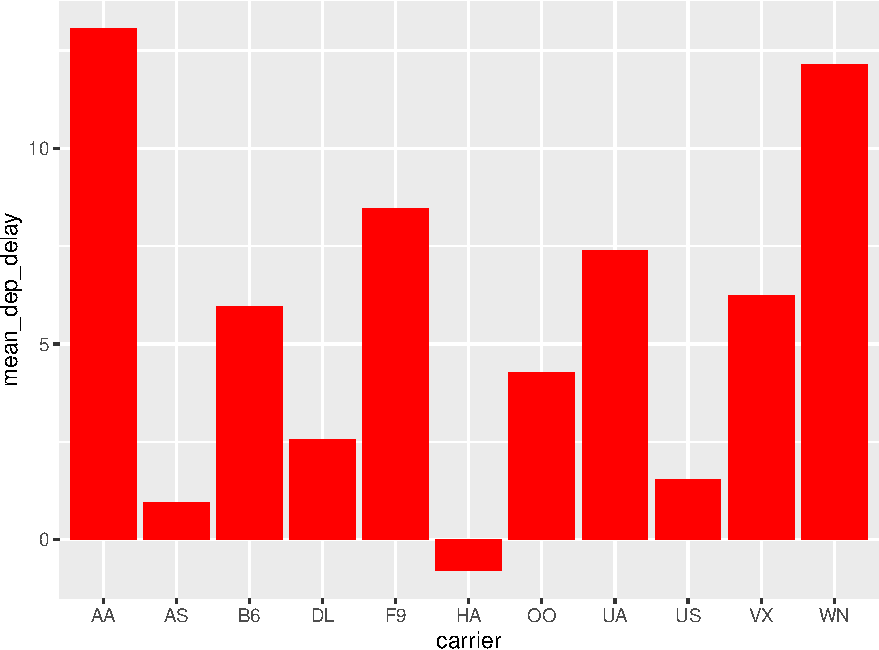
\includegraphics{thesis_files/figure-latex/delaysboxplot-1.pdf}
\caption{\label{fig:delaysboxplot}Mean Delays by Airline}
\end{figure}
Here is a reference to this image: Figure \ref{fig:delaysboxplot}.

A table linking these carrier codes to airline names is available at \url{https://github.com/ismayc/pnwflights14/blob/master/data/airlines.csv}.

\clearpage

Next, we will explore the use of the \texttt{out.extra} chunk option, which can be used to shrink or expand an image loaded from a file by specifying \texttt{"scale=\ "}. Here we use the mathematical graph stored in the ``subdivision.pdf'' file.
\begin{figure}
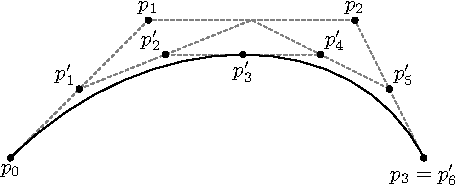
\includegraphics[scale=0.75]{figure/subdivision} \caption{Subdiv. graph}\label{fig:subd}
\end{figure}
Here is a reference to this image: Figure \ref{fig:subd}. Note that \texttt{echo=FALSE} is specified so that the \textbf{R} code is hidden in the document.

\textbf{More Figure Stuff}

Lastly, we will explore how to rotate and enlarge figures using the \texttt{out.extra} chunk option. (Currently this only works in the PDF version of the book.)
\begin{figure}
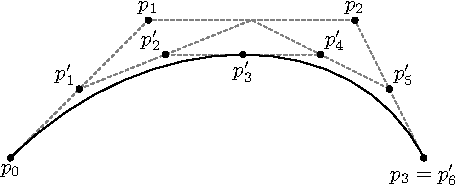
\includegraphics[angle=180, scale=1.1]{figure/subdivision} \caption{A Larger Figure, Flipped Upside Down}\label{fig:subd2}
\end{figure}
As another example, here is a reference: Figure \ref{fig:subd2}.

\hypertarget{footnotes-and-endnotes}{%
\section{Footnotes and Endnotes}\label{footnotes-and-endnotes}}

You might want to footnote something.\footnote{footnote text} The footnote will be in a smaller font and placed appropriately. Endnotes work in much the same way. More information can be found about both on the CUS site or feel free to reach out to \href{mailto:data@reed.edu}{\nolinkurl{data@reed.edu}}.

\hypertarget{bibliographies}{%
\section{Bibliographies}\label{bibliographies}}

Of course you will need to cite things, and you will probably accumulate an armful of sources. There are a variety of tools available for creating a bibliography database (stored with the .bib extension). In addition to BibTeX suggested below, you may want to consider using the free and easy-to-use tool called Zotero. The Reed librarians have created Zotero documentation at \url{http://libguides.reed.edu/citation/zotero}. In addition, a tutorial is available from Middlebury College at \url{http://sites.middlebury.edu/zoteromiddlebury/}.

\emph{R Markdown} uses \emph{pandoc} (\url{http://pandoc.org/}) to build its bibliographies. One nice caveat of this is that you won't have to do a second compile to load in references as standard LaTeX requires. To cite references in your thesis (after creating your bibliography database), place the reference name inside square brackets and precede it by the ``at'' symbol. For example, here's a reference to a book about worrying: (Molina \& Borkovec, 1994). This \texttt{Molina1994} entry appears in a file called \texttt{thesis.bib} in the \texttt{bib} folder. This bibliography database file was created by a program called BibTeX. You can call this file something else if you like (look at the YAML header in the main .Rmd file) and, by default, is to placed in the \texttt{bib} folder.

For more information about BibTeX and bibliographies, see our CUS site (\url{http://web.reed.edu/cis/help/latex/index.html})\footnote{Reed~College (2007)}. There are three pages on this topic: \emph{bibtex} (which talks about using BibTeX, at \url{http://web.reed.edu/cis/help/latex/bibtex.html}), \emph{bibtexstyles} (about how to find and use the bibliography style that best suits your needs, at \url{http://web.reed.edu/cis/help/latex/bibtexstyles.html}) and \emph{bibman} (which covers how to make and maintain a bibliography by hand, without BibTeX, at \url{http://web.reed.edu/cis/help/latex/bibman.html}). The last page will not be useful unless you have only a few sources.

If you look at the YAML header at the top of the main .Rmd file you can see that we can specify the style of the bibliography by referencing the appropriate csl file. You can download a variety of different style files at \url{https://www.zotero.org/styles}. Make sure to download the file into the csl folder.

\textbf{Tips for Bibliographies}
\begin{itemize}
\tightlist
\item
  Like with thesis formatting, the sooner you start compiling your bibliography for something as large as thesis, the better. Typing in source after source is mind-numbing enough; do you really want to do it for hours on end in late April? Think of it as procrastination.
\item
  The cite key (a citation's label) needs to be unique from the other entries.
\item
  When you have more than one author or editor, you need to separate each author's name by the word ``and'' e.g. \texttt{Author\ =\ \{Noble,\ Sam\ and\ Youngberg,\ Jessica\},}.
\item
  Bibliographies made using BibTeX (whether manually or using a manager) accept LaTeX markup, so you can italicize and add symbols as necessary.
\item
  To force capitalization in an article title or where all lowercase is generally used, bracket the capital letter in curly braces.
\item
  You can add a Reed Thesis citation\footnote{Noble (2002)} option. The best way to do this is to use the phdthesis type of citation, and use the optional ``type'' field to enter ``Reed thesis'' or ``Undergraduate thesis.''
\end{itemize}
\hypertarget{anything-else}{%
\section{Anything else?}\label{anything-else}}

If you'd like to see examples of other things in this template, please contact the Data @ Reed team (email \href{mailto:data@reed.edu}{\nolinkurl{data@reed.edu}}) with your suggestions. We love to see people using \emph{R Markdown} for their theses, and are happy to help.

\hypertarget{conclusion}{%
\chapter*{Conclusion}\label{conclusion}}
\addcontentsline{toc}{chapter}{Conclusion}

If we don't want Conclusion to have a chapter number next to it, we can add the \texttt{\{-\}} attribute.

\textbf{More info}

And here's some other random info: the first paragraph after a chapter title or section head \emph{shouldn't be} indented, because indents are to tell the reader that you're starting a new paragraph. Since that's obvious after a chapter or section title, proper typesetting doesn't add an indent there.

\appendix

\hypertarget{the-first-appendix}{%
\chapter{The First Appendix}\label{the-first-appendix}}

This first appendix includes all of the R chunks of code that were hidden throughout the document (using the \texttt{include\ =\ FALSE} chunk tag) to help with readibility and/or setup.

\textbf{In the main Rmd file}
\begin{Shaded}
\begin{Highlighting}[]
\CommentTok{# This chunk ensures that the thesisdown package is}
\CommentTok{# installed and loaded. This thesisdown package includes}
\CommentTok{# the template files for the thesis.}
\ControlFlowTok{if}\NormalTok{(}\OperatorTok{!}\KeywordTok{require}\NormalTok{(devtools))}
  \KeywordTok{install.packages}\NormalTok{(}\StringTok{"devtools"}\NormalTok{, }\DataTypeTok{repos =} \StringTok{"http://cran.rstudio.com"}\NormalTok{)}
\ControlFlowTok{if}\NormalTok{(}\OperatorTok{!}\KeywordTok{require}\NormalTok{(thesisdown))}
\NormalTok{  devtools}\OperatorTok{::}\KeywordTok{install_github}\NormalTok{(}\StringTok{"ismayc/thesisdown"}\NormalTok{)}
\KeywordTok{library}\NormalTok{(thesisdown)}
\end{Highlighting}
\end{Shaded}
\textbf{In Chapter \ref{ref-labels}:}
\begin{Shaded}
\begin{Highlighting}[]
\CommentTok{# This chunk ensures that the thesisdown package is}
\CommentTok{# installed and loaded. This thesisdown package includes}
\CommentTok{# the template files for the thesis and also two functions}
\CommentTok{# used for labeling and referencing}
\ControlFlowTok{if}\NormalTok{(}\OperatorTok{!}\KeywordTok{require}\NormalTok{(devtools))}
  \KeywordTok{install.packages}\NormalTok{(}\StringTok{"devtools"}\NormalTok{, }\DataTypeTok{repos =} \StringTok{"http://cran.rstudio.com"}\NormalTok{)}
\ControlFlowTok{if}\NormalTok{(}\OperatorTok{!}\KeywordTok{require}\NormalTok{(dplyr))}
    \KeywordTok{install.packages}\NormalTok{(}\StringTok{"dplyr"}\NormalTok{, }\DataTypeTok{repos =} \StringTok{"http://cran.rstudio.com"}\NormalTok{)}
\ControlFlowTok{if}\NormalTok{(}\OperatorTok{!}\KeywordTok{require}\NormalTok{(ggplot2))}
    \KeywordTok{install.packages}\NormalTok{(}\StringTok{"ggplot2"}\NormalTok{, }\DataTypeTok{repos =} \StringTok{"http://cran.rstudio.com"}\NormalTok{)}
\ControlFlowTok{if}\NormalTok{(}\OperatorTok{!}\KeywordTok{require}\NormalTok{(ggplot2))}
    \KeywordTok{install.packages}\NormalTok{(}\StringTok{"bookdown"}\NormalTok{, }\DataTypeTok{repos =} \StringTok{"http://cran.rstudio.com"}\NormalTok{)}
\ControlFlowTok{if}\NormalTok{(}\OperatorTok{!}\KeywordTok{require}\NormalTok{(thesisdown))\{}
  \KeywordTok{library}\NormalTok{(devtools)}
\NormalTok{  devtools}\OperatorTok{::}\KeywordTok{install_github}\NormalTok{(}\StringTok{"ismayc/thesisdown"}\NormalTok{)}
\NormalTok{  \}}
\KeywordTok{library}\NormalTok{(thesisdown)}
\NormalTok{flights <-}\StringTok{ }\KeywordTok{read.csv}\NormalTok{(}\StringTok{"data/flights.csv"}\NormalTok{)}
\end{Highlighting}
\end{Shaded}
\hypertarget{the-second-appendix-for-fun}{%
\chapter{The Second Appendix, for Fun}\label{the-second-appendix-for-fun}}

\backmatter

\hypertarget{references}{%
\chapter*{References}\label{references}}
\addcontentsline{toc}{chapter}{References}

\markboth{References}{References}

\noindent

\setlength{\parindent}{-0.20in}
\setlength{\leftskip}{0.20in}
\setlength{\parskip}{8pt}

\hypertarget{refs}{}
\leavevmode\hypertarget{ref-angel2000}{}%
Angel, E. (2000). \emph{Interactive computer graphics : A top-down approach with opengl}. Boston, MA: Addison Wesley Longman.

\leavevmode\hypertarget{ref-angel2001}{}%
Angel, E. (2001a). \emph{Batch-file computer graphics : A bottom-up approach with quicktime}. Boston, MA: Wesley Addison Longman.

\leavevmode\hypertarget{ref-angel2002a}{}%
Angel, E. (2001b). \emph{Test second book by angel}. Boston, MA: Wesley Addison Longman.

\leavevmode\hypertarget{ref-Molina1994}{}%
Molina, S. T., \& Borkovec, T. D. (1994). The Penn State worry questionnaire: Psychometric properties and associated characteristics. In G. C. L. Davey \& F. Tallis (Eds.), \emph{Worrying: Perspectives on theory, assessment and treatment} (pp. 265--283). New York: Wiley.

\leavevmode\hypertarget{ref-noble2002}{}%
Noble, S. G. (2002). \emph{Turning images into simple line-art} (Undergraduate thesis). Reed College.

\leavevmode\hypertarget{ref-reedweb2007}{}%
Reed~College. (2007). LaTeX your document. Retrieved from \url{http://web.reed.edu/cis/help/LaTeX/index.html}


% Index?

\end{document}
